\scanpage{57}
\mspage{\handwritten{24.}}
% archive sheet number: 56

it is therefore a matter of showing that $K$ is affine.

\deleted{The theorem is known in the case where $k$ is algebraically closed\unsure{,} and where $G$ and $H$ are reduced (Chevalley}\deleted{\unsure{)}}\inserted{\deleted{\handwritten{Let us first suppose.}}}
\margin{\figure{\handwritten{
\begin{tikzpicture}[x=0.4cm,y=0.4cm]\draw (0,0) ellipse (3.1 and 0.9);\node at (0,0) {SEE OPPOSITE};\draw (-3,0) .. controls (-5,-1) and (-7,-0.4) .. (-8,-0.4);\draw[->] (-8,-0.35)--(-6.9,-0.5);\draw[gray,thin] (-7.6,.45).. controls (-8,-.1) and (-7.3,-.1)..(-7.65,-.35);\end{tikzpicture}}}}

In the case where $k$ is algebraically closed, and $G$ and $H$ arbitrary,\deleted{(\unsure{$(G/H)_{\mathrm{red}}$} is isomorphic to \unsure{$G_{\mathrm{red}}/H_{\mathrm{red}}$} reduced (\unsure{9.2 vi|9.2 iv})}, $(G\handwritten{\times}_k H)_{\mathrm{red}}$ is isomorphic to $(G_{\mathrm{red}})\handwritten{\times}_k(H_{\mathrm{red}})$, hence $(G_{\mathrm{red}})/(H_{\mathrm{red}})$ is isomorphic to $(G/H)_{\mathrm{red}}$. Since $(G_{\mathrm{red}})/H_{\mathrm{red}}$ is affine, the same is true of $G/H$ (EGA I 5.1.10), for, since $G/H$ is of finite type over $k$, its nilradical is nilpotent.

In the case where $k$ is arbitrary, $G\handwritten{\otimes}_k\handwritten{\bar{k}}/H\handwritten{\unsure{\oslash|\otimes}}_k\handwritten{\bar{k}}$ is isomorphic to $(G/H)\handwritten{\otimes}_k\handwritten{\bar{k}}$ (9.2 v)), hence since the former is affine, the same is true of the latter, hence $G/H$ is affine\handwritten{(ref.)\unsure{'|,}}
\margin{\handwritten{(\qquad)}}

\uline{Second case} : \handwritten{G}eneral case . By (11.13), the algebra $A$ of $G$ is the inductive limit of an increasing filtered family $(A_i)_{i\in I}$ of subalgebras of finite type of $A$ stable under the diagonal map and the involution. By (\deleted{Exp.}\inserted{EGA} I 4.2.3), $H$ is affine, and if we denote the algebra of $H$ by $B$, the homomorphism $A\handwritten{\longrightarrow}B$ deduced from the injection $H\handwritten{\longrightarrow}G$ is surjective. Set $I=\operatorname{Ker}(A\handwritten{\to}B)$, $I_i=I\handwritten{\cap}A_i$ and $B_i=A_i/I_i$; since the associative augmented involutive hyperalgebra structure of $A$ passes to the quotient through $I$, one easily checks that that of $A_i$ passes to the quotient through $I_i$, so that $B_i$ is the algebra of an affine $k$-group of finite type $H_i$; it is clear that $B=\lim B_i$. By (EGA I 4.2.3), $H_i$ is isomorphic to a closed subg\inserted{\handwritten{r\begin{tikzpicture}[x=1cm,y=1cm,baseline=-.1cm]\draw[thin] (-.25,.05)--(-.18,-.3).. controls (-.03,-.12) and (.17,-.17)..(.25,-.1);\end{tikzpicture}}}oup prescheme of $G_i$. By (6.7) the fact that $H$ is invariant in $G$ is expressed by saying that a certain morphism $H\handwritten{\times}_k G\handwritten{\longrightarrow}G$ factors through the injection $H\handwritten{\longrightarrow}G$, in other words that the corresponding homomorphism $A\handwritten{\longrightarrow}B\handwritten{\otimes}_k A$ factors through the canonical homomorphism $A\handwritten{\longrightarrow}B$; one easily checks that the homomorphism $A_i\handwritten{\longrightarrow}B_i\handwritten{\otimes}_k A_i$ defined analogously factors through $A_i\handwritten{\longrightarrow}B_i$, hence that $H_i$ is invariant in $G_i$. By what was seen previously, $G_i$ being of finite type over\inserted{\handwritten{\ \begin{tikzpicture}[x=1cm,y=1cm,baseline=0cm]\draw[thin] (0,.3)--(-.03,-.35);\end{tikzpicture}}}$k$, $G_i/H_i$ is representable by an affine $k$-group $K_i$, whose algebra we shall denote by $C_i$. Set th\deleted{e}\handwritten{\unsure{e|4}}n $C=\underset{\handwritten{\longrightarrow}}{\lim}C_i$, and let $K=\underset{\handwritten{\longleftarrow}}{\lim}K_i$ be the affine $k$-prescheme with algebra $K$ (EGA IV 8.2.3).

\margin{\figure{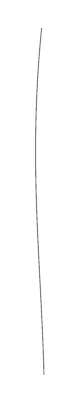
\begin{tikzpicture}[x=1cm,y=1cm]\draw[gray,thin] (0,0).. controls (-.04,1.5) and (-.2,2.7)..(-.03,4.4);\end{tikzpicture}}}

Let us show that $K$ represents $G/H$; for this, it suffices to verify that \deleted{the diagram}
\margin{\handwritten{is this defined ?}}
\diagram{\begin{tikzcd}[ampersand replacement=\&,execute at end picture={\draw[thin] (current bounding box.center) ellipse [x radius=4.2cm,y radius=0.55cm];}]
H\handwritten{\times}_k G \arrow[r,"\handwritten{\sim}"] \& G\deleted{\unsure{\longrightarrow K}}\handwritten{\times_K G}\quad\text{\deleted{is Cartesian}}
\end{tikzcd}}
\handwritten{,} and that the morphism $G\handwritten{\longrightarrow}K$ is covering for the fpqc topology. (\deleted{\unsure{Exp.}} IV 4.4.3). Now, \deleted{each of the diagrams}\inserted{\handwritten{for each $i$, one \unsure{-|has}}}
\diagram{\begin{tikzcd}[ampersand replacement=\&]
H_i\handwritten{\times}_k G_i \arrow[r,"\handwritten{\sim}"] \& G_i\deleted{\unsure{\longrightarrow K_i}}\handwritten{\times_{K_i}G_i}
\end{tikzcd}}
\handwritten{,}\deleted{being Cartesian,}\inserted{\handwritten{thus}} the same is true o\deleted{\unsure{f the|f}}\handwritten{f the} \deleted{diagram}\inserted{\handwritten{morphism\begin{tikzpicture}[x=1cm,y=1cm,baseline=-.1cm]\draw[thin] (0,.06).. controls (.18,-.15) and (-.85,-.1)..(-.9,-.3)--(-.85,-.47);\end{tikzpicture}}} obtained by passing to the projective limit; finally each of the morphisms
